\documentclass[10pt,aspectratio=169]{beamer}
\usepackage[utf8]{inputenc}
\usepackage[english]{babel}
\usepackage{xcolor}
\usepackage{amsmath}
\usepackage{amssymb}
\usepackage{bm}
\usepackage{csquotes}
\usepackage{mathtools}
\usepackage{graphicx}
\usepackage{tikz}
\usetikzlibrary{positioning,arrows.meta}
\usepackage{booktabs}
\usepackage[backend=biber,sorting=nyt,natbib=true,style=authoryear,maxcitenames=2,maxbibnames=99]{biblatex}
\addbibresource{ref.bib}

\title[Antitrust \& Competition]{Tackling Competition Issues with Advanced Methods}

\author[Z. Wang]{Zhongli Wang}

\institute{Bielefeld University; Università Cattolica del Sacro Cuore} 

\date{\today}

\usetheme[
  lelofont=false,
  smallmargins,
  authorinfoot,
  titleinfoot,
  totalframes,
  mylogoinfoot=false,
  logoinfoot=false,
  department=none,
  departmentlang=none,
  institutelang=none
]{IMW}

\begin{document}

\begin{frame}
  \vfill
  \begin{center}
    {\usebeamerfont{title}\usebeamercolor[fg]{title}\inserttitle\par}
    \vspace{1.4em}
    {\small\itshape E.CA Interview \par}
    \vspace{0.8em}
    {\usebeamerfont{author}\insertauthor\par}
    \vspace{0.8em}
    {\usebeamerfont{institute}\insertinstitute\par}
    \vspace{0.8em}
    {\usebeamerfont{date}\insertdate\par}
    \vspace{0.8em}
    
\includegraphics[width=0.82\textwidth]{logos/epoc_logo_0002.png}
  \end{center}
  \vfill
\end{frame}

% \begin{frame}{Outline}
%   \tableofcontents
% \end{frame}

\begin{frame}{My Research: Five Papers}
  \begin{block}{Research Portfolio}
    \begin{itemize}
      \item \textbf{P1 -- Data Restrictions \& Competition:} How data privacy regulations shape firm strategies and market structures in software markets
      \item \textbf{P2 -- Capacity \& Network Effects:} Strategic service capacity investment under congestion and consumer networks in ICT markets (Job Market Paper)
      \item \textbf{P3 -- ABM Calibration:} Parameter estimation methods using real telecom data (AT\&T, T-Mobile)
      \item \textbf{P4 -- Financial Fraud Detection:} Polytope Fraud Theory using supervised learning (\textit{Int. Rev. Financial Analysis}, 2025)
      \item \textbf{P5 -- AI in Economics:} Agentic workflows for economic research using LLMs and multimodal AI (arXiv)
    \end{itemize}
  \end{block}
\end{frame}

\begin{frame}{Skills for Competition Economics}
  \begin{alertblock}{Methodological Expertise}
    \begin{itemize}
      \item \textbf{Agent-Based Modeling:} Design, implementation (Python/Julia/R), and calibration of complex economic systems
      % \item \textbf{Regulation as Parameters:} Modeling how firm learning and adaptation shape agent behavior and market outcomes through parameter adjustments
      \item \textbf{Counterfactual Policy Analysis:} Evaluating policy interventions under heterogeneity and feedback mechanisms
      \item \textbf{Machine Learning:} Pattern detection in complex data using supervised learning (XGBoost, Neural Networks, Random Forest)
      \item \textbf{Empirical Calibration:} Simulated Method of Moments, neural network surrogates, and validation techniques
    \end{itemize}
  \end{alertblock}
\end{frame}

% \section{About My Research}

\begin{frame}{Research Methodology Framework}
  \begin{block}{Empirical Rigor Across All Papers}
    Each research project follows a disciplined four-stage process:
    \begin{enumerate}
      \item \textbf{Hypothesis Formation:} Identify market failures, regulatory gaps, or strategic puzzles from theory and real-world observations
      \item \textbf{Data Collection:} Gather empirical evidence from firm reports, regulatory databases, financial markets, or experimental simulations
      \item \textbf{Statistical Analysis:} Apply econometric methods, machine learning, or agent-based modeling to test hypotheses
      \item \textbf{Findings Interpretation:} Translate results into policy implications and strategic insights
    \end{enumerate}
  \end{block}
\end{frame}

\begin{frame}{Paper 2: Capacity Investment \& Network Effects (JMP)}
  \begin{block}{Hypothesis Formation}
    \textbf{RQ:} How do service capacity constraints, congestion, and consumer networks jointly shape firm competition in ICT markets?
    \\
    \textbf{Theory:} Network effects amplify user-base advantages, but congestion degrades quality unless firms invest sufficiently in capacity
  \end{block}

  \begin{block}{Data Collection}
    \begin{itemize}
      \item ICT market characteristics: network effects, congestion patterns, capacity constraints
      \item Consumer behavior: small-world network structure, information diffusion, switching decisions
      \item Firm strategies: pricing, physical R\&D investment, capacity management
    \end{itemize}
  \end{block}
\end{frame}

\begin{frame}{Paper 2: Capacity Investment \& Network Effects (cont.)}
  \begin{block}{Statistical Analysis}
    % \textbf{Methods:}
    \begin{itemize}
      \item Agent-based computational model with duopoly competition
      \item Network dynamics: small-world topology with information diffusion
      \item Firm heuristics: myopic profit-based investment adjustments
      % \item Quality function: $\theta_{i,t} = A_i - \beta_2 \max(0, m_{i,t} - \chi_{i,t})$ (congestion penalty)
    \end{itemize}
  \end{block}

  \begin{alertblock}{Findings Interpretation}
    \begin{itemize}
      \item Capacity is a quality driver and differentiation tool, not just production constraint
      \item Network effects amplify market concentration; congestion limits dominant firm profitability
      \item Technological edge enables dominance; smaller firms compete via pricing flexibility
      \item Frequent investment $\neq$ higher profits; strategic timing matters
    \end{itemize}
  \end{alertblock}
\end{frame}

\begin{frame}{Paper 2: Network Structure}
  \begin{figure}
    \centering
    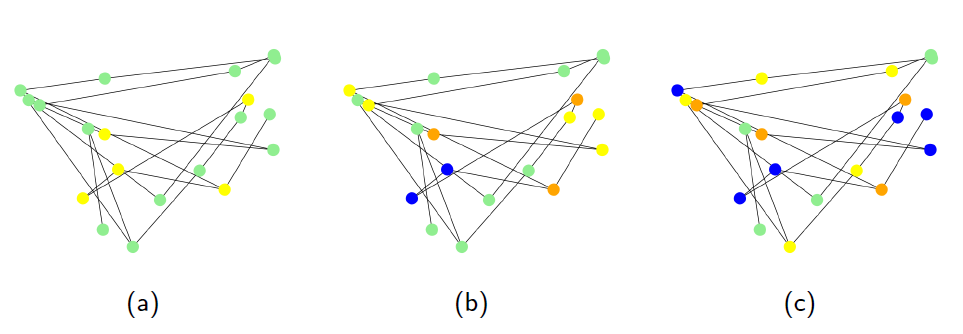
\includegraphics[width=0.8\textwidth]{nw.png}
    \caption{Small-world network structure enabling consumer information diffusion}
  \end{figure}
\end{frame}

\begin{frame}{Paper 2: Market Dynamics Simulation (1)}
  \begin{figure}
    \centering
    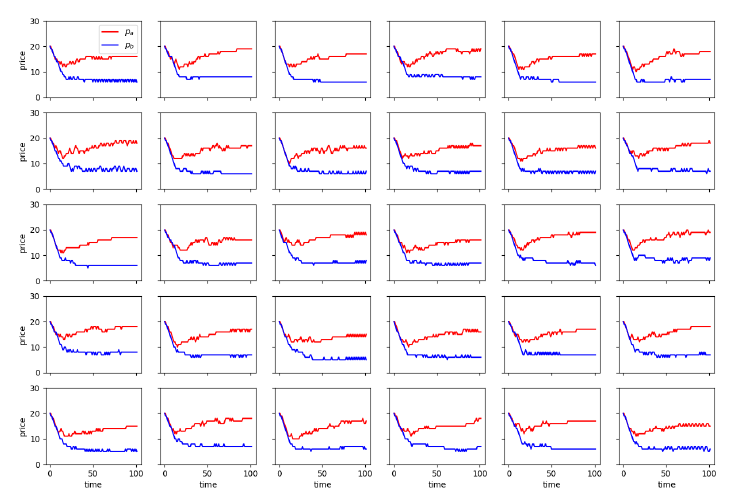
\includegraphics[width=0.6\textwidth]{simul1.png}
    \caption{Time series of product prices}
  \end{figure}
\end{frame}

\begin{frame}{Paper 2: Market Dynamics Simulation (2)}
  \begin{figure}
    \centering
    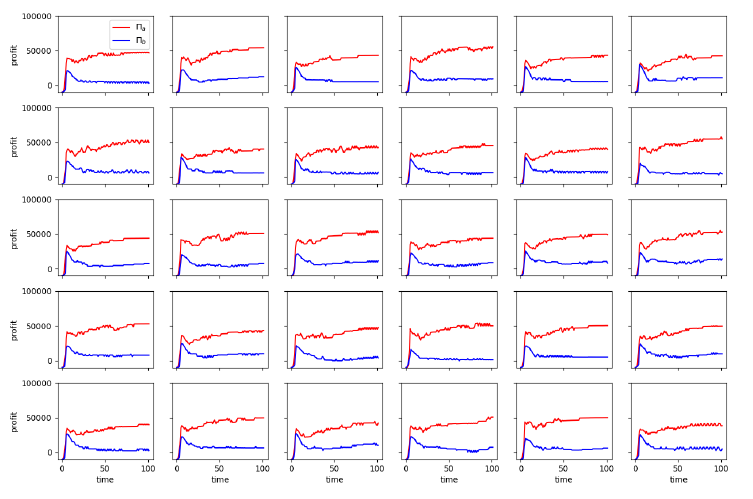
\includegraphics[width=0.6\textwidth]{simul2.png}
    \caption{Time series of firm profits}
  \end{figure}
\end{frame}

\begin{frame}{Paper 1: Data Restrictions \& Competition}
  \begin{block}{Hypothesis Formation}
    \textbf{RQ:} How do varying levels of data privacy regulations influence price formation and market structures in software markets?
    \\
    \textbf{Theory:} Data restrictions act as both compliance costs and product attributes (privacy-conscious consumers value restrictions)
  \end{block}

  \begin{block}{Data Collection}
    \begin{itemize}
      \item Stylized regional regulatory environments (low vs. high data restriction)
      \item Consumer preference distributions (functionality vs. privacy trade-offs)
      \item Firm cost structures (fixed R\&D investment, variable compliance costs)
    \end{itemize}
  \end{block}
\end{frame}

\begin{frame}{Paper 1: Data Restrictions \& Competition (cont.)}
  \begin{block}{Statistical Analysis}
    % \textbf{Methods:}
    \begin{itemize}
      \item Game-theoretic equilibrium analysis (two-stage investment-pricing game)
      \item Agent-based simulations with heterogeneous consumers (Hotelling framework)
      \item Counterfactual scenarios across regulatory regimes
    \end{itemize}
  \end{block}

  \begin{alertblock}{Findings Interpretation}
    \begin{itemize}
      \item Consumer taste distribution determines competitive outcomes: indifferent consumers $\rightarrow$ low-restriction firm dominates; privacy-conscious consumers $\rightarrow$ intense competition
      \item Cross-regional regulatory cooperation increases both consumer welfare and firm profits
      \item Regional differentiation in restrictions benefits both firms through product differentiation
    \end{itemize}
  \end{alertblock}
\end{frame}

\begin{frame}{Paper 3: ABM Calibration with Real Telecom Data}
  \begin{block}{Hypothesis Formation}
    \textbf{RQ:} Which estimation techniques are most suitable for calibrating agent-based models to real-world data?
    \\
    \textbf{Theory:} ABM credibility requires empirical grounding; parameter estimation remains a major methodological challenge
  \end{block}

  \begin{block}{Data Collection}
    \begin{itemize}
      \item U.S. telecom sector: AT\&T vs. T-Mobile (2019-2023)
      \item Firm-level data: revenue, subscribers, costs, profits (monthly frequency)
      \item Sources: Official firm reports, Statista, Refinitiv
      \item Temporal disaggregation: annual/quarterly $\rightarrow$ monthly
    \end{itemize}
  \end{block}
\end{frame}

\begin{frame}{Paper 3: ABM Calibration with Real Telecom Data (cont.)}
  \begin{block}{Statistical Analysis}
    % \textbf{Methods:}
    \begin{itemize}
      \item Simulated Method of Moments (SMM): minimize NRMSE between simulated and empirical moments
      \item Neural Network Surrogate: maps 21 parameters $\rightarrow$ loss function; enables gradient-based optimization
      \item Latin Hypercube Sampling for parameter space exploration (16 target parameters)
    \end{itemize}
  \end{block}

  \begin{alertblock}{Findings Interpretation}
    \begin{itemize}
      \item SMM and NN surrogate are complementary: SMM matches moments; NN enables efficient re-use and gradient search
      \item Price-adjustment parameter identified as most influential for firm control
      \item Calibrated model reproduces observed market dynamics, confirming empirical relevance
      % \item Non-stationarity and path dependence limit full validation but partial fit achieved
    \end{itemize}
  \end{alertblock}
\end{frame}

\begin{frame}{Paper 4: Polytope Fraud Theory}
  \begin{block}{Hypothesis Formation}
    \textbf{RQ:} Can financial statement fraud be reliably detected using public accounting data and machine learning?
    \\
    \textbf{Theory:} Activist short sellers identify fraud patterns; these signals can be formalized as financial red flags
  \end{block}

  \begin{block}{Data Collection}
    \begin{itemize}
      \item Manually labeled dataset: activist short sellers' targets (fraudulent firms)
      \item Control group: non-fraudulent firms matched by industry and size
      \item Financial metrics: 10 red flags derived from short-seller behavior (cash flow anomalies, revenue quality, etc.)
      \item Public financial statements from SEC filings
    \end{itemize}
  \end{block}
\end{frame}

\begin{frame}{Paper 4: Polytope Fraud Theory (cont.)}
  \begin{block}{Statistical Analysis}
    % \textbf{Methods:}
    \begin{itemize}
      \item Supervised learning: Random Forest, Neural Networks, XGBoost
      \item Feature engineering: 10 financial red flags as predictors
      \item Cross-validation and out-of-sample testing
      \item Model interpretation: feature importance analysis
    \end{itemize}
  \end{block}

  \begin{alertblock}{Findings Interpretation}
    \begin{itemize}
      \item XGBoost achieves strong performance: 72\% recall, 82\% F1-score
      \item Ten financial red flags reliably identify fraudulent firms
      \item Published in \textit{International Review of Financial Analysis} (2025)
      \item Investors and regulators can use these signals for early fraud detection
    \end{itemize}
  \end{alertblock}
\end{frame}

\begin{frame}{Paper 5: Agentic Workflows in Economic Research}
  \begin{block}{Hypothesis Formation}
    \textbf{RQ:} Can Large Language Models and multimodal AI automate tasks across the economic research lifecycle?
    \\
    \textbf{Theory:} Specialized AI agents with human-in-the-loop oversight can enhance efficiency and reproducibility
  \end{block}

  \begin{block}{Data Collection \& Implementation}
    \begin{itemize}
      \item Framework design: agentic workflow combining LLMs and multimodal AI
      \item Implementation: Microsoft AutoGen with specialized agents
      \item Tasks: literature review, data analysis, empirical modeling, visualization
      \item Human oversight: validation checkpoints at each stage
    \end{itemize}
  \end{block}
\end{frame}

\begin{frame}{Paper 5: Agentic Workflows in Economic Research (cont.)}
  \begin{block}{Statistical Analysis}
    % \textbf{Methods:}
    \begin{itemize}
      \item Multi-agent system design with task decomposition
      \item Workflow orchestration: sequential and parallel agent execution
      \item Quality control: human validation at critical decision points
    \end{itemize}
  \end{block}

  \begin{alertblock}{Findings Interpretation}
    \begin{itemize}
      \item Agentic workflows can automate routine research tasks while maintaining rigor
      \item Human-in-the-loop oversight essential for methodological validity
      \item Enhances reproducibility and efficiency in economic research
      \item Demonstrates practical implementation
    \end{itemize}
  \end{alertblock}
\end{frame}

\begin{frame}{Summary: Why This Matters for Competition Economics}
  \begin{itemize}
    \item \textbf{Methodological toolkit:} ABM + ML + empirical calibration
    \item \textbf{Policy-relevant insights:} Regulation, market structure, firm strategy
    \item \textbf{Proven track record:} Published research with real-world applications
    \item \textbf{Ready to contribute:} Applying the methods to real competition cases
  \end{itemize}
\end{frame}
\end{document}
